\documentclass[pdf, aspectratio=169]{beamer}
\usepackage[]{hyperref,graphicx,siunitx,lmodern,booktabs,tikz,tensor}
\usepackage{pgfplots,pgfplotstable}
\usepackage{pdfpc-commands}

\usepackage[mode=buildnew]{standalone}
\mode<presentation>{\usetheme{Astro}}

\graphicspath{ {../Images/} }

\sisetup{per-mode=symbol}
\usetikzlibrary{calc,angles,quotes, intersections, decorations.pathmorphing,shadings}
\tikzstyle{proton}=[circle, minimum size = 7mm, ball color=red, black,transform shape]
\tikzstyle{neutron}=[circle, minimum size=7mm, ball color=gray, black, transform shape]
\tikzstyle{gammaray}=[ultra thick, -latex, decorate, decoration={snake, post length=3mm}]

\pgfdeclarehorizontalshading{startype}{100bp}{
  color(0bp)=(black!50!red);
  color(25bp)=(black!50!red);
  color(28bp)=(red);
  color(32bp)=(orange);
  color(36bp)=(yellow);
  color(40bp)=(white);
  color(50bp)=(cyan!50);
  color(60bp)=(cyan!50!blue);
  color(70bp)=(blue);
  color(75bp)=(blue!50!violet!70!black);
  color(100bp)=(blue!50!violet!50!black)
}

%preamble
\title{You are all so bright!}
\date{October 29, 2018}
\author{Jed Rembold}

\begin{document}
\renewcommand*{\theenumi}{\Alph{enumi}}

\begin{frame}{Announcements}
  \begin{itemize}
	  \item Back to the grind: WebWorK due on Wednesday
	  \item I should be able to hand tests back on Wednesday or Friday
	  \item No lab this week!
		  \begin{itemize}
			  \item If you have a lab to make-up, \alert{this is the week to do it}!
			  \item Email me with what lab you want to be making up please!
		  \end{itemize}
	\item Poll: \url{rembold-class.ddns.net}
  \end{itemize}
\end{frame}


\begin{frame}{In the Sky}
	\begin{itemize}
		\item Moon in waning gibbous
		\item Jupiter and Mercury hanging out together just after sunset
			\begin{itemize}
				\item Should be able to see them both in the same field-of-view when using binoculars
			\end{itemize}
		\item Saturn and Mars still up through much of the night
		\item Iridium Flare: Oct 30 at 6:00:36pm towards the West (mag=-7)
		\item ISS crossings:
			\begin{itemize}
				\item Oct 30 at 7:07am (mag=-3.3)
				\item Oct 31 at 6:17am (mag=-3.8)
			\end{itemize}
		\item 0 sunspots on the Sun currently!
	\end{itemize}
\end{frame}

\begin{frame}{Review Question!}
  It takes energy thousands of years to travel from the interior of the Sun to Earth because:
  \begin{enumerate}
	\item The Earth is a really long way away
	\item Neutrino's interfere with the gamma rays, slowing them down
	\item \alert<2>{Lots of collisions with charged particles slow  and scatter the gamma rays}
	\item Neutrino's carry the bulk of the energy and travel much slower than light
  \end{enumerate}

\end{frame}

%\begin{frame}{Flareon}
  %\begin{itemize}
	%\item Most flares occur near sunspots, implying a connection to the magnetic field
	%\item Unlike the Earth, the equator of the Sun rotates faster than the poles!
	  %\begin{itemize}
		%\item Think tradewinds on Earth, but the entire Sun is a gas
	  %\end{itemize}
	%\item Gases tend to drag the magnetic field with them
	%\item Things can get very tangled, and flares are though to be a way of rearranging magnetic field lines to untangle them
  %\end{itemize}
  %\begin{center}
	%\inlineMovie{../Videos/Flare.ogv}{../Videos/Flare.png}{width=.5\textwidth}
  %\end{center}
%\end{frame}

%\begin{frame}{Effects on Earth}
  %\begin{itemize}
	%\item Communications
	%\item Aurora
  %\end{itemize}
  %\begin{center}
	%\includegraphics[height=4cm]{ch11_aurora_ground.jpg}
	%\includegraphics[height=4cm]{ch11_aurora_space.jpg}
  %\end{center}
%\end{frame}

%\fullFrameImage{ch11_solar_cycle.jpg}

\fullFrameImageZoomed{ch12_starrynight.jpg}

\begin{frame}{What can we directly observe?}
  \begin{itemize}
	\item The light from the stars tells us:
	  \begin{itemize}
		\item Their location in the sky
		\item The intensity of their light
		\item Their spectrum
	  \end{itemize}
	\item From these, we can determine:
	  \begin{itemize}
		\item Surface Temperature
		\item Motion
		\item Distance (sometimes)
		\item Size (in a way)
		\item Power output (Luminosity)
		\item Mass (also sometimes)
	  \end{itemize}
  \end{itemize}
\end{frame}

\begin{frame}{A note on Angular Size}
  \begin{columns}
	\column{.5\textwidth}
	\begin{itemize}
	  \item Recall that the angular size of the Sun is about \SI{0.5}{\degree}
		\begin{itemize}
		  \item Angular sizes of stars much, much smaller
		  \item Generally smaller than can be resolved with any telescope
		\end{itemize}
	  \item Main exception: Betelgeuse
		\begin{itemize}
		  \item HST measured an angular size of 0.07 arcseconds
		  \item Equal to 20 millionth of a degree
		\end{itemize}
	\end{itemize}
	\column{.5\textwidth}
	\begin{center}
	  \includegraphics[width=.7\textwidth]{ch12_Betelgeuse.jpg}
	\end{center}
  \end{columns}
\end{frame}

\begin{frame}{Truly Stellar Spectra!}
  \begin{columns}
	\column{.5\textwidth}
	\begin{center}
	  \includegraphics[width=.7\textwidth]{ch12_Betelgeuse.jpg}
	\end{center}
	\column{.5\textwidth}
	\begin{itemize}
	  \item Stars come in a wide variety of colors
	  \item These colors correspond to surface temperatures of $\approx$~\SIrange{3000}{50000}{\kelvin}
		\begin{itemize}
		  \item Wien's Law
		  \item Stefan-Boltzmann Law
		\end{itemize}
	\end{itemize}
  \end{columns}
\end{frame}

\begin{frame}{Just Not My Type}
  \begin{columns}
	\column{.5\textwidth}
	\begin{itemize}
	  \item Stars were originally classified by the strength of their Hydrogen lines
	  \item The strongest were type A, all the way down to Type O
	\end{itemize}
	\column{.5\textwidth}
	\begin{center}
	  \includegraphics[width=.8\textwidth]{ch12_StarTypes.png}
	\end{center}
  \end{columns}
\end{frame}

\begin{frame}{Scrambling the System}
	\begin{itemize}
	  \item As more star spectra observed, H lines were inadequate
	  \item Annie Cannon
		\begin{itemize}
		  \item Classified some 350,000 stars (yeesh)
		  \item A new order based on Balmer lines, not alphabetical this time
		  \item Some classes overlapped and could be eliminated
		\end{itemize}
	  \item Mnenomics
		\begin{itemize}
		  \item Oh, Be A Fine Girl/Guy, Kiss Me
		  \item Only Boring Astronomers Find Gratification Knowing Mnemonics
		\end{itemize}
	\end{itemize}
	\begin{center}
	  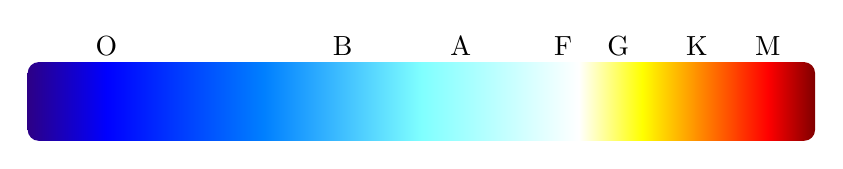
\begin{tikzpicture}
		\shade[rounded corners,shading=startype, shading angle=180] (0,0) rectangle +(10,1);
		\node at (1,1.2) {O};
		\node at (4,1.2) {B};
		\node at (5.5,1.2) {A};
		\node at (6.8,1.2) {F};
		\node at (7.5,1.2) {G};
		\node at (8.5,1.2) {K};
		\node at (9.4,1.2) {M};
	  \end{tikzpicture}
	\end{center}
\end{frame}

\begin{frame}{It is Apparent!}
  \begin{columns}
	\column{.5\textwidth}
	\begin{itemize}
	  \item Apparent Brightness is the intensity of radiation from the star
		\begin{itemize}
		  \item As measured from the Earth's surface
		  \item Units of Watts/$m^2$
		\end{itemize}
	  \item For the Sun $B\approx \SI{1400}{\watt\per\meter^2}$
	  \item This is much, much less for other stars
	  \item The traditional unit of apparent brightness is \alert{apparent magnitude}
	\end{itemize}
	\column{.5\textwidth}
	\begin{center}
	  \begin{tikzpicture}
		\clip (0,0) circle (2.54cm);
		\node at (0,0) {\includegraphics[width=\textwidth]{ch12_LightFalloff.png}};
	  \end{tikzpicture}
	\end{center}
  \end{columns}
\end{frame}

\begin{frame}{The Apparent Magnitude}
  \begin{itemize}
	\item System introduced around 150 BC
	\item Hipparchus divided stars into six groups:
	  \begin{itemize}
		\item Brightest were ``1st magnitude''
		\item Faintest (that he could see) were ``6th magnitude''
	  \end{itemize}
	\item These days we are much more precise:
	  \begin{itemize}
		\item 1st magnitude about 2.5 times brighter than 2nd
		\item 2nd is about 2.5 times brighter than 3rd
		\item Happens with a logarithmic scale!
		  \begin{itemize}
			\item A factor of 100 in brightness is a difference of 5 in magnitude
		  \end{itemize}
	  \end{itemize}
  \end{itemize}
  \[m = -2.5\log\left( \frac{B_{obj}}{B_{Vega}} \right)\]
\end{frame}

\begin{frame}{Making Sense of Magnitudes}
  \begin{itemize}
	\item Smaller numbers mean brighter stars
	\item Numbers can be negative
	\item Smaller differences in magnitude correspond to larger differences in brightness
  \end{itemize}
  \begin{center}
	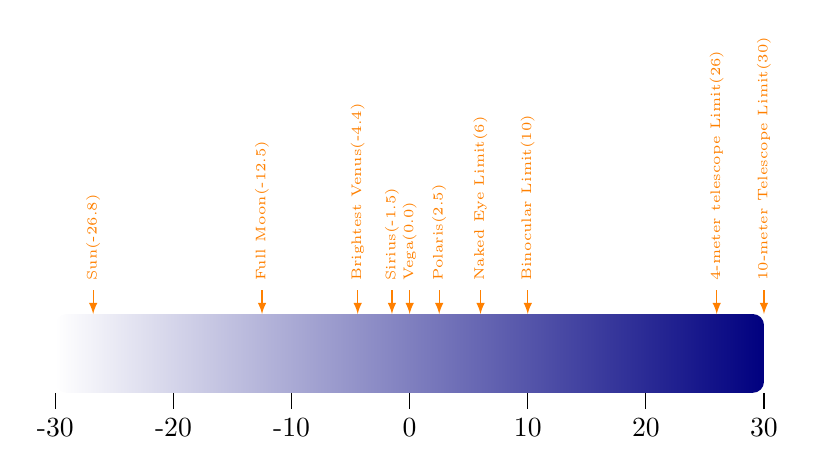
\begin{tikzpicture}[xscale=.15, lbl/.style={rotate=90,right,font=\tiny}]
	  \shade[rounded corners, left color=white, right color=black!50!blue] (-30,0) rectangle +(60,1);
	  \foreach \e in {-30,-20,...,30}{
		\draw (\e,0) --+(0,-2mm) node[below] {\e};
	  }
	  \draw[orange,latex-] (-26.8,1) --+(0,3mm) node[lbl] {Sun(-26.8)};
	  \draw[orange,latex-] (-12.5,1) --+(0,3mm) node[lbl] {Full Moon(-12.5)};
	  \draw[orange,latex-] (-4.4,1) --+(0,3mm) node[lbl] {Brightest Venus(-4.4)};
	  \draw[orange,latex-] (-1.5,1) --+(0,3mm) node[lbl] {Sirius(-1.5)};
	  \draw[orange,latex-] (0.0,1) --+(0,3mm) node[lbl] {Vega(0.0)};
	  \draw[orange,latex-] (2.5,1) --+(0,3mm) node[lbl] {Polaris(2.5)};
	  \draw[orange,latex-] (6,1) --+(0,3mm) node[lbl] {Naked Eye Limit(6)};
	  \draw[orange,latex-] (10,1) --+(0,3mm) node[lbl] {Binocular Limit(10)};
	  \draw[orange,latex-] (26,1) --+(0,3mm) node[lbl] {4-meter telescope Limit(26)};
	  \draw[orange,latex-] (30,1) --+(0,3mm) node[lbl] {10-meter Telescope Limit(30)};
	\end{tikzpicture}
  \end{center}
\end{frame}

\begin{frame}{Magnitude Example}
  \begin{example}
	I measure a nearby star to be 500 times brighter than the star Vega. What is the apparent magnitude of said star?
  \end{example}
\end{frame}

\begin{frame}{Flipping the Tables}
  \begin{itemize}
	\item What if you want to go the other direction?
	\item Know two magnitudes and want to figure out how much brighter one object is than the other
	  \[\frac{B_1}{B_2} = 10^{0.4 \times (m_2-m_1)}\]
  \end{itemize}
\end{frame}

\begin{frame}{Reverse Example}
  \begin{example}
	One of the Iridium Flares for tomorrow is to have an apparent magnitude of -7.0. How many times dimmer is this than the brightness of the full moon?
  \end{example}
\end{frame}

%\begin{frame}{Understanding Check!}
  %Jupiter is 12 times brighter than Vega while Venus is approximately 60 times brighter than Vega. What is the difference between the apparent magnitudes of Jupiter and Venus ($m_V - m_J$)
  %\begin{enumerate}
	%\item \alert<2>{-1.7}
	%\item -0.7
	%\item 0.2
	%\item 5
  %\end{enumerate}
%\end{frame}

\begin{frame}{Luminosity}
  \begin{columns}
	\column{.5\textwidth}
	\begin{itemize}
	  \item We measure the apparent brightness $B$
	  \item Brightness falls off with distance:
		\[B = \frac{L}{4\pi d^2}\]
	  \item Thus the luminosity is
		\[L = 4\pi d^2 \times B\]
	  \item Range of stellar luminosities is large:
		\begin{itemize}
		  \item $L_{Sun}$ = \SI{4e26}{\watt}
		  \item Dimmest at $0.000001 L_{Sun}$
		  \item Brightest at $100000 L_{Sun}$
		\end{itemize}
	\end{itemize}
	\column{.5\textwidth}
	\begin{center}
	  \begin{tikzpicture}
		\clip (0,0) circle (2.54cm);
		\node at (0,0) {\includegraphics[width=\textwidth]{ch12_LightFalloff.png}};
	  \end{tikzpicture}
	\end{center}
  \end{columns}
\end{frame}

%\begin{frame}{Star Sizes}
  %\begin{itemize}
	%\item We've mentioned that we can \emph{not} resolve most stars
	%\item We can get the size in a sneaky way though!
	  %\begin{itemize}
		%\item Stefan-Boltzmann law and Luminosity:
		  %\begin{align*}
			%L &= 4\pi R^2 \times I \\
			%&= 4\pi R^2 \times \sigma T^4
		  %\end{align*}
	  %\end{itemize}
	%\item A \textcolor{red!70!black}{cooler} star can have a high luminosity if it is {\LARGE large}
	%\item A \textcolor{blue!40}{hot} star can have a low luminosity if it is {\scriptsize small}
  %\end{itemize}
%\end{frame}

\begin{frame}{Refresher}
  We wanted to be able to find:
	\begin{itemize}
	  \item \alert<2->{Surface Temperature}
	  \item \alert<2->{Motion}
	  \item Distance (sometimes)
	  \item {Size (in a way)}
	  \item \alert<3->{Power output (Luminosity)}
	  \item Mass (also sometimes)
	\end{itemize}
\end{frame}

%\begin{frame}{Stellar Distances}
  %\begin{itemize}
	%\item Back to parallax!
	%\item Still the only real method we have to determine distances to stars
	%\item Recall parallax effects are larger for closer objects
	  %\begin{itemize}
		%\item We need as large a baseline as we can get: observe during 6 month intervals
		%\item The parallax effects from stars are still tiny!
		%\item Generally less than an arcsecond
	  %\end{itemize}
	%\item A \alert{Parsec} is the distance that corresponds to a parallax angle of 1 arcsecond
	  %\begin{itemize}
		%\item Equivalent to 3.26 light years
	  %\end{itemize}
	%\item Measuring the parallax angle ($p$) in arcseconds yields
	  %\[d = \frac{1}{p}\]
	  %where $d$ is in parsecs. 
  %\end{itemize}
%\end{frame}



\end{document}
